\vspace{-0.2cm}
\section{Impact of Sampling Error and Overfitting}
\label{sec:overfitting}
\vspace{-0.2cm}

\begin{wrapfigure}{r}{0.35\linewidth}
    \centering
    \vspace{-20pt}
    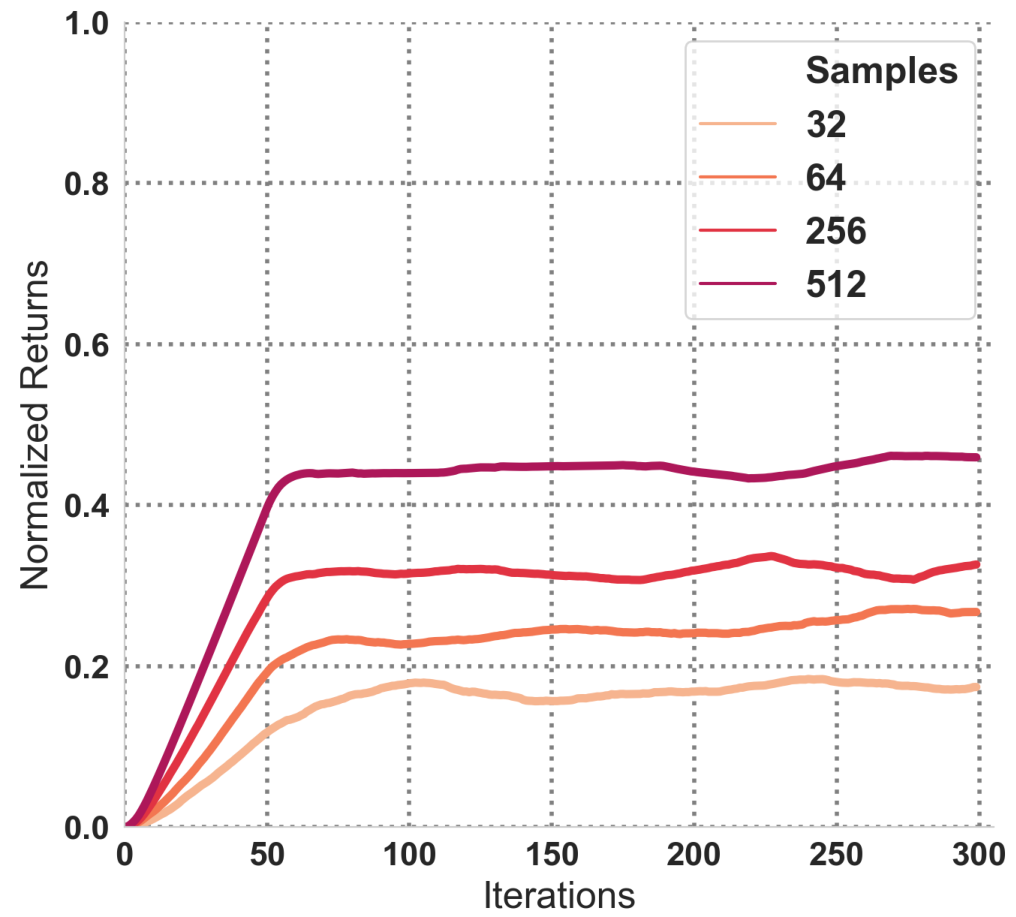
\includegraphics[width=0.8\linewidth]{chapters/diagnosing_q/images/samples_arch.pdf}
    \vspace{-0.2cm}
    \caption{\label{fig:sampling_256} Samples vs. returns. More samples yields better performance.}
    \vspace{-0.6cm}
    %plot_sampling
    %east1//2019-01-20-newenv-sample-weighting
\end{wrapfigure}
So far, we have observed that the performance of off-policy RL algorithms based on Q-learning can be quite sensitive to the distribution of the offline data, even when all the transition tuples in the MDP are provided to the algorithm, and only the weighting over these samples is varied. In this section, we aim to study a distinct question: we investigate the performance of off-policy Q-learning when the offline dataset is of a finite size and may not contain all transitions in the MDP. To address any confounders from distributional shift, we provide the underlying Q-learning algorithm oracle access to collecting data from the current snapshot of the learned policy. While this sort of active data collection is not possible in the offline RL problem setting, this simplification allows us to more carefully localize the challenges of overfitting and sampling error.

We analyze several key points that relate to sampling error. First, we show that Q-learning is prone to overfitting, and this overfitting has a real impact on performance.
% So far, we observed that the performance of off-policy RL algorithms based on Q-learning can be quite sensitive to the distribution of the offline data, even when all the transition tuples in the MDP are provided to the algorithm, and only the weighting over these samples is varied. In this section, we aim to study a distinct question: we study the performance of off-policy Q-learning when the offline dataset is of a finite size, and may not contain all transitions in the MDP. To address any confounders from distributional shift, we provide the underlying Q-learning algorithm oracle access to collecting data from the current snapshot of the learned policy. While this sort of active data collection is not possible in the offline RL problem setting, this simplification allows us to more carefully localize the challenges of overfitting and sampling error.

% We analyze several key points that relate to sampling error. First, we show that Q-learning is prone to overfitting, and that this overfitting has a real impact on performance. 

\vspace{-0.2cm}
\subsection{Quantifying Overfitting}
\vspace{-0.2cm}
We first quantify the amount of overfitting during training, by varying the number of samples. In order provide comparable validation errors across different experiments, we fix a reference sequence of Q-functions, $Q^1, ... , Q^N$, obtained during an arbitrary run of Q-learning. We then retrace the training sequence, and minimize the projection error $\Projmu(Q^t)$ at each training iteration, using varying amounts of on-policy data or sampling from a replay buffer. We measure the validation error (the expected Bellman error) at each iteration under the on-policy distribution, plotted in Figure~\ref{fig:sampling_validation_loss}. We note the obvious trend that more samples leads to significantly lower validation loss. 
% A more interesting observation is that sampling from the replay buffer results in the lowest on-policy validation loss, despite bias due to distribution mismatch from sampling off-policy data. As we elaborate in Section~\ref{sec:analysis_nonstationarity}, we believe that replay buffers are effective because they reduce overfitting and have good sample coverage over the state space, not necessarily due to reducing the effects of nonstationarity.

Next, Figure~\ref{fig:sampling_256} shows the relationship between number of samples and returns. We see that more samples leads to improved learning speed and a better final solution. Despite overfitting being an issue, larger architectures still perform better because the bias introduced by smaller architectures dominates. This observation indicate that the nature of overfitting in RL is likely significantly different from that of supervised learning: while overfitting in supervised learning can bne controlled by regulating model capacity, off-policy RL methods likely need to rely on alternative techniques to control overfitting. We made some progress towards understanding this questions in \citet{li2023efficient}.   

\begin{figure*}[ttt!]
\begin{subfigure}{0.31\linewidth}
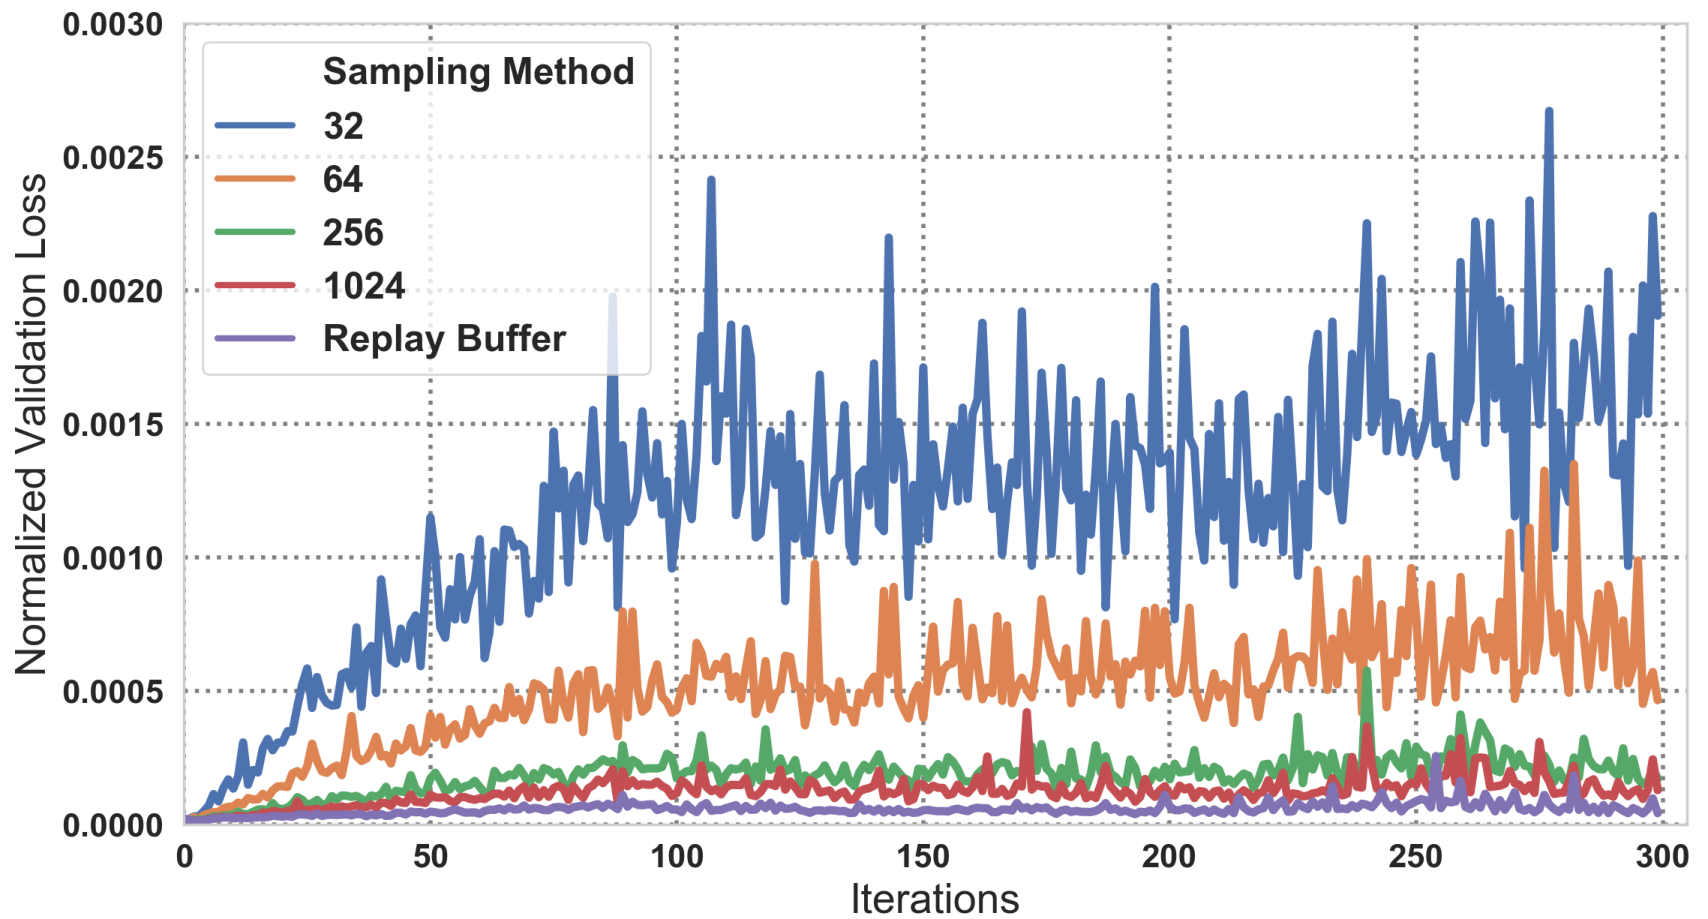
\includegraphics[width=0.97\linewidth]{chapters/diagnosing_q/images/overfitting.pdf}
%plot_overfitting
%central1//2019-01-21-overfitting-coupled
\caption{\label{fig:sampling_validation_loss} On-policy validation losses for varying amounts of on-policy data (or replay buffer), averaged across environments and seeds. Note that sampling from the replay buffer has lower on-policy validation loss, despite bias from distribution shift.}
\end{subfigure}
~\vline~
\begin{subfigure}{0.31\linewidth}
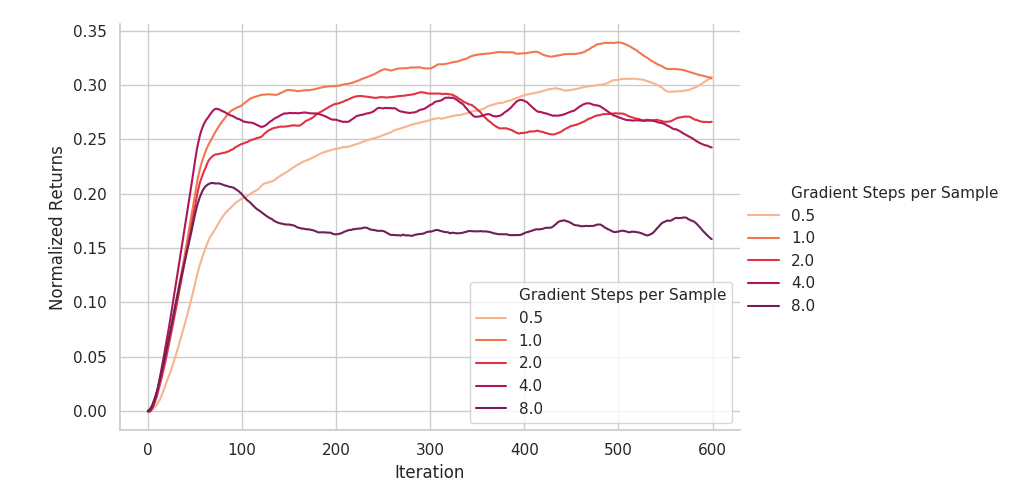
\includegraphics[trim={0 0 7.0cm 0},clip,width=0.97\linewidth]{chapters/diagnosing_q/images/grad_steps_fqi}
%plot_overfitting
%central1//2019-01-21-overfitting-coupled
\caption{\label{fig:fqi_grad_sweep}Normalized returns plotted over training iterations (32 samples per iteration), for different ratios of gradient steps per sample. We observe that intermediate values of gradient steps work best, and too many gradient steps hurt performance.}
\end{subfigure}
~\vline~
\begin{subfigure}{0.31\linewidth}
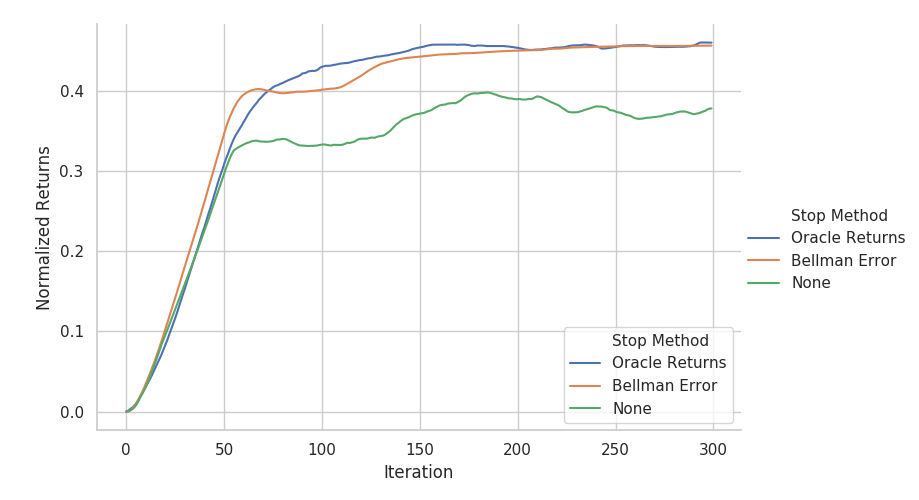
\includegraphics[trim={0 0 4.4cm 0},clip,width=0.97\linewidth]{chapters/diagnosing_q/images/validation_stop}
%plot_validation_stop
%west1//2019-02-20-replay-validation-stop
\caption{\label{fig:validation_stop}Normalized returns plotted over training iterations (32 samples are taken per iteration), for different early stopping methods. We observe that using proper early stopping can result in a modest performance increase.}
\end{subfigure}
\end{figure*}

\vspace{-0.2cm}
\subsection{Does Compensating for Overfitting Improve Performance?}
\vspace{-0.2cm}

Finally, to confirm our hypotheses regarding overfitting, we now wish to understand if compensating for overfitting does lead to improved performance. One common technique for reducing overfitting is to utilize \textit{early stopping} methods to mitigate overfitting without reducing model size.
% We first note that the number of gradient steps taken per sample in the projection step has an important effect on performance -- too few steps and the algorithm learns slowly, but too many steps and the algorithm may initially learn quickly but overfit. To show this, we run an ablation over the number of gradient steps taken per sample in Replay-FQI and TD3 (TD3 uses 1 by default). Results for FQI are shown in Fig.~\ref{fig:fqi_grad_sweep}, and for TD3 in Appendix Fig.~\ref{fig:td3_grad_sweep}.
In order to understand whether early stopping criteria can reduce overfitting, we employ \emph{oracle} stopping rules to provide an ``upper bound'' on the best potential improvement. We try two criteria for setting the number of gradient steps: the expected Bellman error and the expected returns of the greedy policy (oracle returns). We implement both methods by minimizing the TD-error to convergence, and retroactively selecting the intermediate Q-function which is judged best by the evaluation metric. Using oracle stopping metrics results in a modest boost in performance in tabular domains (Fig.~\ref{fig:validation_stop}). Thus, we believe that there is promise in further improving such early-stopping methods for reducing overfitting in deep RL algorithms.

\textbf{To summarize}, we can draw a few conclusions from our experiments in this section. First, overfitting is indeed an issue with Q-learning, and too many gradient steps or too few samples can lead to poor performance. Second, although overfitting is a problem, large architectures are still preferred, because the bias from function approximation outweighs the increased overfitting from using large models. 

Finally, we also remark that attempting to learn optimal policies from a static offline dataset will present both distributional shift and overfitting challenges together, and we would expect these to be tightly coupled with each other in the following sense: the inability to correclty identify the underlying MDP from finite samples in the offline dataset will induce errors in policy optimization, and these errors would then be exacerbated in the next step of learning as the learned policy deviates from the training data. This will also be evident in the theoretical results that we will present in subsequent chapters.    